\documentclass[conference]{IEEEtran}
\usepackage{amsmath}
\usepackage{graphicx}
\usepackage{booktabs}
\usepackage{array}
\usepackage{url}
\usepackage[hidelinks]{hyperref}

\begin{document}

\title{Schedule-Aware Learned Rate Control for RDMA Datacenter Fabrics Carrying Distributed AI Training Traffic: Implementation and Experimental Evaluation}

\author{
\IEEEauthorblockN{Abdul Samad}
\IEEEauthorblockA{BS Artificial Intelligence, FAST NUCES Islamabad \\
Registration No. 24I-0095 \\
i240095@isb.nu.edu.pk}
}

\maketitle

\begin{abstract}
Distributed AI training sends data in short synchronized bursts that repeat every step, and one slow flow can stall a whole collective. Existing RDMA congestion control schemes react after queues build up and use fixed parameters. In this phase we implement and test a rate controller that anchors each sender at its expected fair share and then applies a small learned correction. The controller is a 121 parameter network trained with evolution strategies, and the work includes a burst forecaster for other jobs. We build a flow level simulator, re-implement DCQCN, HPCC, Barre and ACC style baselines in it, and test on 40 random and 40 shifted scenarios plus four named ones. Our controller lowers the mean collective completion time slowdown by @@G_DC@@\% against DCQCN and @@G_BA@@\% against the Barre style controller, and almost removes PFC pauses. We also report negative findings. A hand written rule that knows the job schedule is statistically tied with the learned controller on completion time, and forecasting other jobs' compute time gave no measurable benefit.
\end{abstract}

\begin{IEEEkeywords}
RDMA, congestion control, collective communication, distributed training, evolution strategies, datacenter networks
\end{IEEEkeywords}

\section{Introduction}
Phase 1 and Phase 2 reviewed eleven recent papers on RDMA congestion control and load balancing for AI clusters. The same weaknesses appeared again and again. Controllers react late, their constants are set by hand, they are rarely tested with collective traffic, and they are judged by flow completion time instead of training step time. Phase 2 proposed a predictive learned controller to address this.

This report is the Phase 3 implementation. It follows the seven items of the handout. We describe the implementation and the changes to the Phase 2 plan, the data and preprocessing, the baselines, the graphical results, a comparison with published work, the ablations, and a critical discussion. Several of our Phase 2 expectations were only partly confirmed, and we say so where it happens.

\section{Implementation of the Methodology}

\subsection{Simulator}
We wrote a flow level simulator in Python with Numba. Time is advanced in steps of 5 $\mu$s. All senders share one 100 Gbps bottleneck with a FIFO queue, a feedback delay of 20 $\mu$s, ECN marking between 100 KB and 400 KB with a maximum probability of 0.2, and PFC with a pause threshold of 1.5 MB and a resume threshold of 1.0 MB. The network is lossless. Each job runs a repeating loop of a compute phase and a communication phase. A communication phase is a list of steps, and every step starts only when the slowest flow of the previous step has finished. A Ring-AllReduce is $2(n-1)$ steps with $n$ flows each. An AllToAll or mixture of experts exchange is two steps with up to 16 flows. Up to three jobs share the link.

The main quantity we measure is the collective completion time (CCT) of every iteration. We report CCT slowdown, which is the CCT divided by the time the same collective would need alone on the link. In multi-job scenarios the slowdown is above 1 even for a perfect scheduler, because the jobs share one link.

\subsection{Controllers}
\textbf{Baselines.} All baselines run inside the same simulator, so the comparison uses identical dynamics.
\begin{itemize}
\item \textbf{DCQCN:} standard rate decrease by $\alpha/2$ on a congestion notification, fast recovery followed by additive increase, 55 $\mu$s timers, $g=1/16$.
\item \textbf{HPCC style:} once per RTT, the rate is scaled by the measured link utilization against a target of 0.95, plus a small additive step.
\item \textbf{Barre style:} DCQCN structure with a small decrease of 3\% per notification, a fast increase after five increases without congestion, and a cut to one quarter when the delayed queue is above half of the PFC threshold. This is a simplified version of the published design.
\item \textbf{ACC style:} DCQCN with ECN thresholds that are scaled by a rule every 100 $\mu$s, down when the queue is near the PFC level and up when the link is underused.
\end{itemize}

\textbf{Proposed controller.} Each flow gets an anchor rate and a learned correction. The anchor is the fair share $\min(R_{line}, C/\hat n)$, where $\hat n$ is the number of flows expected to be active on the link. $\hat n$ is the job's own active flow count plus the flows of other jobs whose forecast burst window contains the current time. A small network with 8 inputs, 12 tanh hidden units and one output gives a value $a\in[-1,1]$, and the rate is $\text{anchor}\cdot e^{1.5a}$ limited to the allowed range. The policy is evaluated every 20 $\mu$s and immediately when a flow starts. The 8 inputs are the current rate, the ECN mark average, the delayed queue depth, the remaining fraction of the flow, the anchor rate, the expected concurrency 300 $\mu$s ahead, the time since the burst started, and the expected change in concurrency. The policy has @@QP@@ parameters.

We evaluate two versions. \textbf{Ours (predictive)} forecasts the compute time of every job with a small MLP, which gives a predicted burst window for the other jobs. \textbf{Ours (schedule-aware)} only knows the flow count of its own collective, and has no forecast of other jobs. We also test a hand written rule that uses the anchor rate alone without any learning.

\subsection{Burst forecaster}
The forecaster is a lag window MLP with 8 past compute times (divided by their mean) as input and 16 hidden units. It predicts the next compute time of a job. A predicted burst window starts at the forecast time and lasts 1.3 times the ideal collective duration.

\subsection{Training}
The policy is trained with evolution strategies: antithetic sampling with 8 pairs, noise standard deviation 0.1, centered rank shaping and the Adam optimizer with learning rate 0.06, for 30 generations. Each generation uses 6 freshly sampled training scenarios of 8 iterations, shared by all candidates in that generation. The fitness is minus the mean CCT slowdown, minus 0.05 times the percentage of time spent in PFC pause. The parameters with the best validation fitness are kept, using 6 separate validation scenarios. Seven policies were trained, one for each variant used in the ablation.

\subsection{Changes to the Phase 2 methodology}
\begin{table}[t]
\centering
\caption{Differences between the Phase 2 plan and this implementation}
\label{tab:changes}
\scriptsize
\begin{tabular}{p{2.2cm}p{3.0cm}p{2.5cm}}
\toprule
\textbf{Phase 2 plan} & \textbf{Implemented} & \textbf{Reason} \\
\midrule
ASTRA-sim with ns-3, 32 to 256 GPUs & Own flow level simulator, one shared bottleneck, up to 3 jobs & Runs on one CPU core in tens of milliseconds per scenario \\
GRU or TCN predictor & Lag window MLP, 8 inputs & No deep learning framework in the environment \\
PPO or SAC & Evolution strategies & Tiny policy, non-differentiable simulator \\
Distillation and quantization & Quantization only & Policy is already tiny \\
Cross-datacenter family & Dropped & Scope of one semester \\
Burst time forecast as the key idea & Kept, plus a schedule-aware variant & Added after the first tests (see Section VII) \\
\bottomrule
\end{tabular}
\end{table}

\section{Dataset and Preprocessing}
There is no public dataset of collective traffic for this problem, so all data is generated from parameters. This is a limitation that we discuss later.

\textbf{Traffic.} Ring-AllReduce jobs use 4, 6 or 8 flows with 0.5 to 1.5 MB per flow and step. AllToAll jobs use 8, 12 or 16 flows with 2 to 5 MB per flow and two steps. The compute time of a job has a base value between 6 and 20 ms. Each iteration's compute time is the base value times one plus a periodic term (amplitude 0.05 to 0.2, period 2, 3, 4 or 6 iterations), plus first order autoregressive noise (coefficient 0.3 to 0.8, noise level 0.01 to 0.05), with a 4\% chance of a 40\% longer iteration. Times are scaled down so that compute and communication are of similar size.

\textbf{Splits.} Training scenarios are drawn fresh in every generation. Validation uses 6 scenarios (seed 999). The test sets are never used for training. The \emph{random} test set has 40 scenarios from the same family (seed 777). The \emph{shifted} test set has 40 scenarios with periods 5, 7 and 8, stronger autocorrelation 0.8 to 0.95 and noise 0.04 to 0.1, all outside the training range (seed 888). The four named scenarios S1 to S4 each use 10 random seeds. Each run has 14 iterations, and the first 2 are discarded as warm-up.

\textbf{Preprocessing and features.} The forecaster input is normalized by the mean of its window. The policy inputs are scaled to about the range 0 to 2. Queue depth is delayed by the feedback delay, and ECN information is an exponential average of notifications. Phase labels come from the simulator.

\textbf{Forecaster training.} The MLP was trained on 400 generated sequences of 40 iterations from the training family.

\section{Baseline Evaluation}
Table~\ref{tab:main} shows the mean CCT slowdown for all methods and scenario sets, and Table~\ref{tab:detail} gives all metrics on the random test set with 95\% bootstrap confidence intervals for CCT slowdown. S1 is one AllReduce job, S2 is one AllToAll job, S3 has two jobs and S4 has three jobs.

\begin{table}[t]
\centering
\caption{Mean CCT slowdown (lower is better)}
\label{tab:main}
\scriptsize
\begin{tabular}{lcccccc}
\toprule
\textbf{Method} & \textbf{S1} & \textbf{S2} & \textbf{S3} & \textbf{S4} & \textbf{Rand.} & \textbf{Shift.} \\
\midrule
@@MAINTAB@@
\bottomrule
\end{tabular}
\end{table}

\begin{table*}[t]
\centering
\caption{All metrics on the random test set (40 scenarios). Iteration time includes compute time.}
\label{tab:detail}
\small
\begin{tabular}{lccccccc}
\toprule
\textbf{Method} & \textbf{CCT slowdown [95\% CI]} & \textbf{P99} & \textbf{Iter. (ms)} & \textbf{PFC (\%)} & \textbf{Jain} & \textbf{Util.} & \textbf{FCT (ms)} \\
\midrule
@@DETAILTAB@@
\bottomrule
\end{tabular}
\end{table*}

Before using the simulator for comparisons we checked the DCQCN model on a simple test with 8 long flows. The average queue was @@V_Q@@ KB, the link utilization was @@V_U@@ and the Jain fairness index was @@V_J@@ (Fig.~\ref{fig:val}). This shows plausible behaviour but is not a replacement for validation against ns-3.

\begin{figure}[t]
\centering
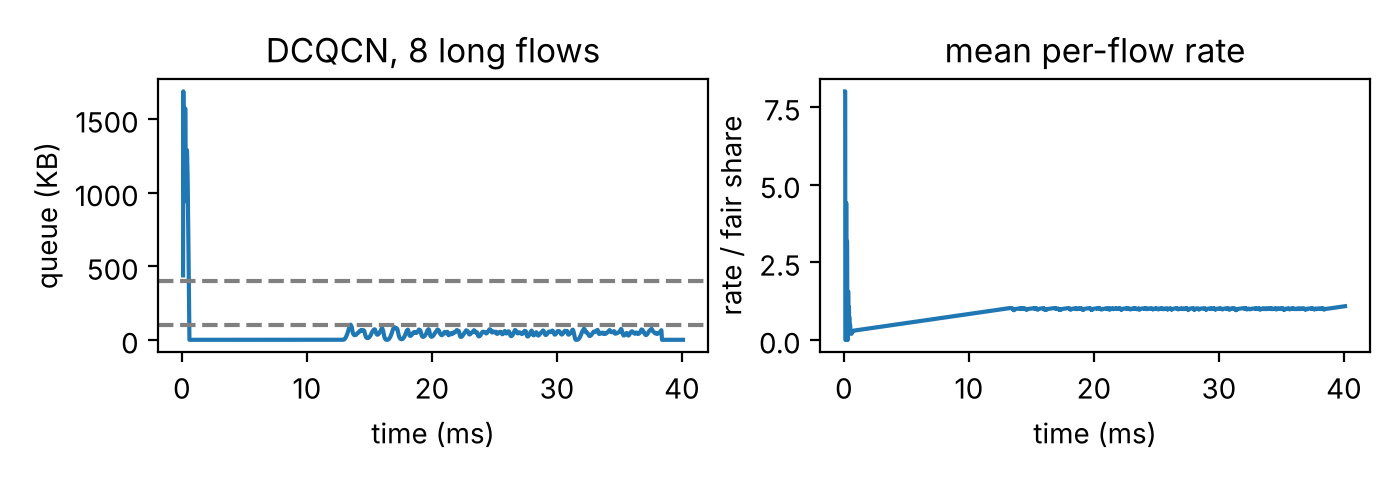
\includegraphics[width=\columnwidth]{figs/validation.png}
\caption{Sanity check of the DCQCN model with 8 long flows. Dashed lines are the ECN thresholds.}
\label{fig:val}
\end{figure}

\section{Graphical Results}
Figure~\ref{fig:main} shows the mean CCT slowdown with 95\% confidence intervals. The existing schemes lose most in the multi-job cases. DCQCN and ACC style waste link capacity after rate cuts, so the last flows of every step finish late. On the random and shifted sets the Barre style controller is the best of the baselines.

\begin{figure*}[t]
\centering
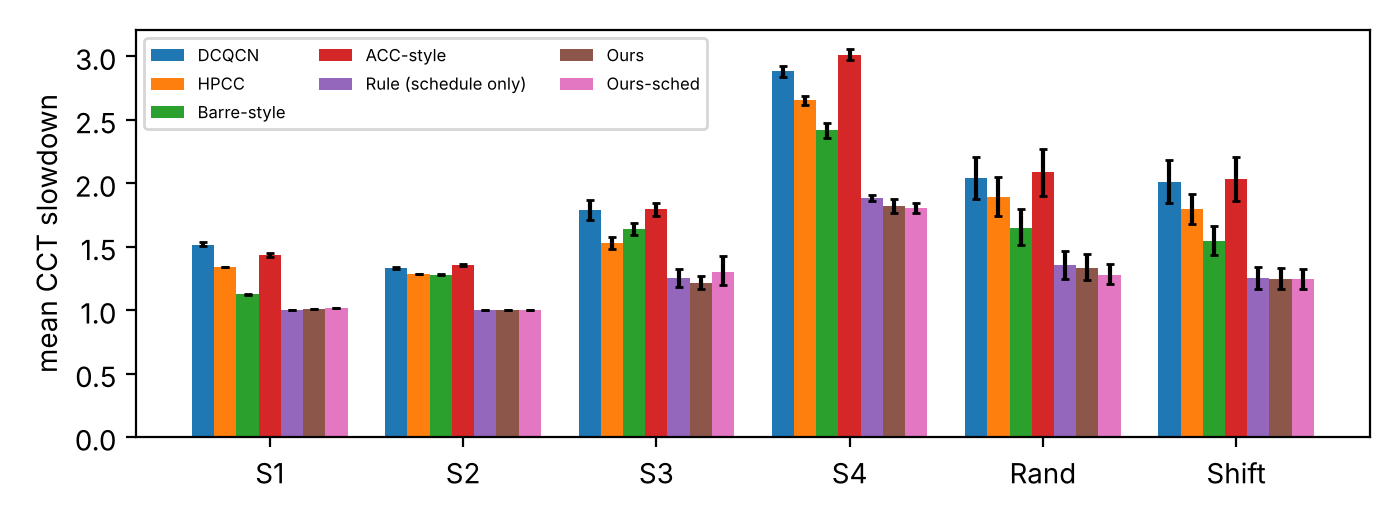
\includegraphics[width=0.85\textwidth]{figs/main_cct.png}
\caption{Mean CCT slowdown on the named scenarios (10 seeds each) and on the random and shifted test sets (40 scenarios each). Error bars are 95\% bootstrap confidence intervals.}
\label{fig:main}
\end{figure*}

Figure~\ref{fig:cdf} shows the distribution over all iterations. The P99 slowdown on the random set is @@P99_DC@@ for DCQCN, @@P99_OURS@@ for our predictive controller and @@P99_SCH@@ for the schedule-aware one. Figure~\ref{fig:trace} shows the first burst of the single AllToAll job S2, where all methods start at the same moment. DCQCN, HPCC style and Barre style all start 16 flows at line rate and overshoot to a peak queue of @@TQ_DC_P@@, @@TQ_HP_P@@ and @@TQ_BA_P@@ KB, above the 1500 KB PFC threshold. Our controller starts at the expected fair share and peaks at @@TQ_O_P@@ KB. After the start, HPCC style keeps the queue almost empty but leaves the link partly idle, while DCQCN and Barre style oscillate. Our controller holds a steady queue of about @@TQ_O_M@@ KB on average (against @@TQ_DC_M@@ KB for DCQCN), which keeps the link fully busy but adds some queueing delay, about 28 $\mu$s at 100 Gbps.

\begin{figure}[t]
\centering
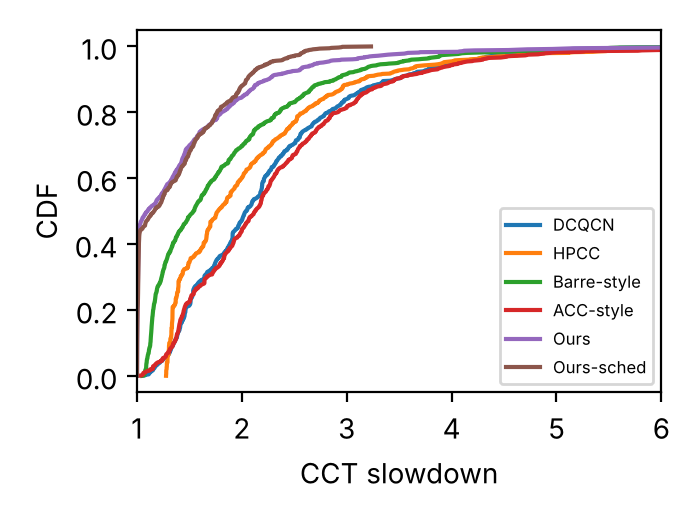
\includegraphics[width=\columnwidth]{figs/cdf.png}
\caption{Distribution of CCT slowdown over all iterations of the random test set.}
\label{fig:cdf}
\end{figure}

\begin{figure}[t]
\centering
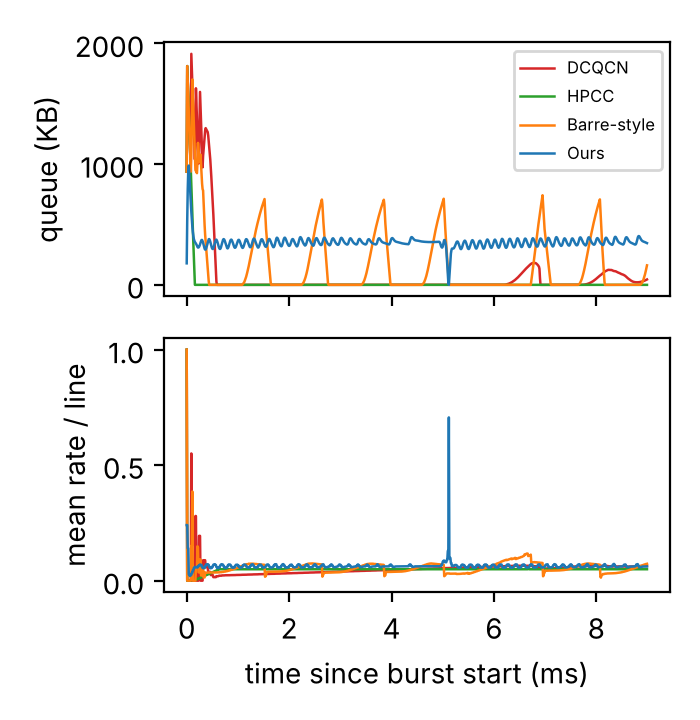
\includegraphics[width=\columnwidth]{figs/trace.png}
\caption{Queue length and mean sender rate around the first burst of the single AllToAll job S2.}
\label{fig:trace}
\end{figure}

\subsection{Statistical comparison}
Table~\ref{tab:stats} gives the mean gain in CCT slowdown and a paired Wilcoxon signed rank test over the 40 scenarios of each test set. Against the four existing schemes the gains are clear and consistent on both sets. Our two versions are not significantly different from each other or from the no-learning rule.

\begin{table}[t]
\centering
\caption{Paired comparison on the two test sets (40 scenarios each)}
\label{tab:stats}
\tiny
\begin{tabular}{llccc}
\toprule
\textbf{Set} & \textbf{Comparison} & \textbf{Gain (\%)} & \textbf{Wins} & \textbf{p} \\
\midrule
@@STATTAB@@
\bottomrule
\end{tabular}
\end{table}

\subsection{Sensitivity}
Figure~\ref{fig:sens} shows three sweeps on random multi-job scenarios. We added noise to the compute time forecasts, scaled the compute time (a smaller compute time means more overlap between jobs), and changed the compute jitter. Our controllers stay ahead of the baselines in all cases. The forecast noise did not change the result of the predictive version: the mean slowdown was @@PN0@@ without noise and @@PN5000@@ with 5000 $\mu$s of error, compared with @@PNDC@@ for DCQCN and @@PNHP@@ for HPCC. With the compute time scaled down to 0.25, the schedule-aware controller reached @@LD025@@ against @@LD025D@@ for DCQCN. With the scale at 2.0 it reached @@LD2@@ against @@LD2D@@.

\begin{figure*}[t]
\centering
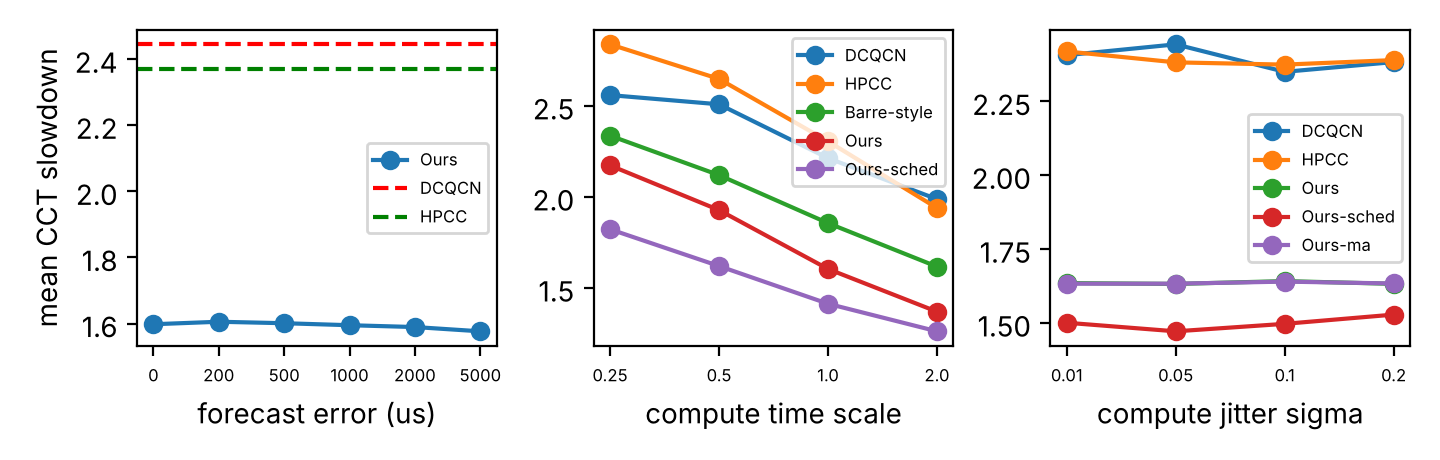
\includegraphics[width=0.9\textwidth]{figs/sensitivity.png}
\caption{Sensitivity of the mean CCT slowdown to forecast error (left), compute time scale (middle) and compute jitter (right) on random multi-job scenarios.}
\label{fig:sens}
\end{figure*}

\subsection{Forecaster and training}
The lag window MLP lowers the forecast error from @@E1MA@@\% (moving average) to @@E1ML@@\% on sequences like the training family. On the shifted family the two are equal (@@E1MAS@@\% and @@E1MLS@@\%), so it does not generalize to stronger autocorrelation. Longer history windows help the forecaster. Figure~\ref{fig:pred} shows the errors and Figure~\ref{fig:train} the validation fitness during training.

\begin{figure}[t]
\centering
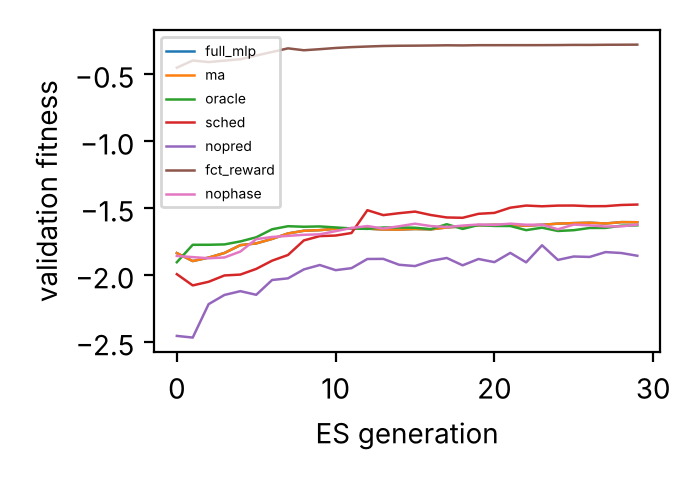
\includegraphics[width=\columnwidth]{figs/training.png}
\caption{Validation fitness of the seven policies during evolution strategies training.}
\label{fig:train}
\end{figure}

\begin{figure}[t]
\centering
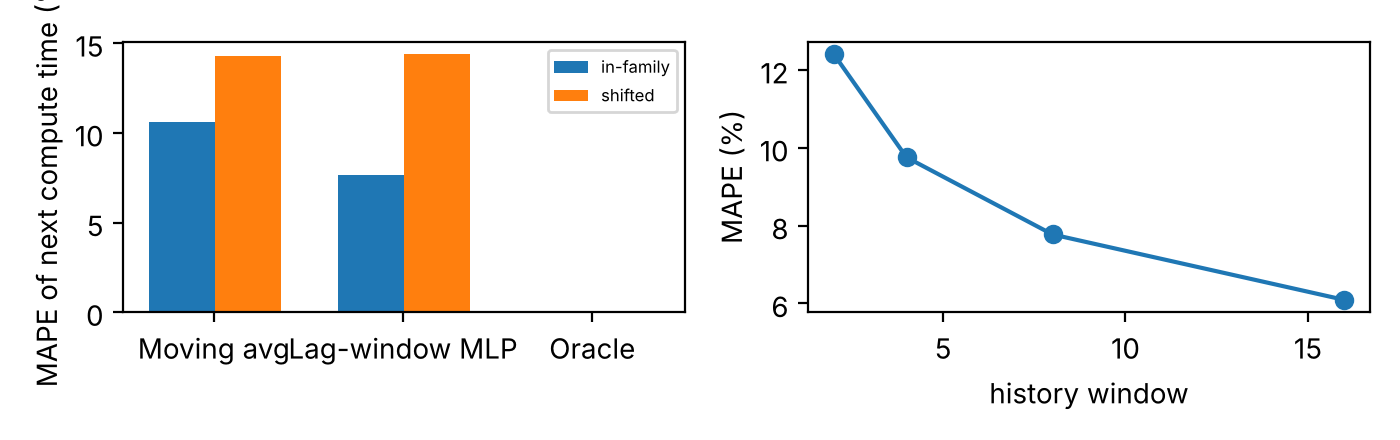
\includegraphics[width=\columnwidth]{figs/predictor.png}
\caption{Forecast error of the moving average, the lag window MLP and an oracle (left), and the effect of the history length (right).}
\label{fig:pred}
\end{figure}

\section{Comparison with Existing Research}
Published numbers come from different settings, so we compare directions and rough sizes, not exact values. Table~\ref{tab:comp} lists them.

\begin{table}[t]
\centering
\caption{Our results next to reported results}
\label{tab:comp}
\scriptsize
\begin{tabular}{p{1.3cm}p{3.2cm}p{2.7cm}}
\toprule
\textbf{Work} & \textbf{Reported result} & \textbf{Ours (simulated)} \\
\midrule
Barre & About 9.6\% higher training throughput and 56\% lower latency than DCQCN on a real 256 GPU AllToAll cluster & CCT of a single AllToAll job @@S2_G@@\% lower than DCQCN (S2); @@G_DC@@\% lower on the random set \\
SPILLWAY & About 5\% shorter iteration time in cross-datacenter training, up to 14\% shorter microbatch & Iteration time @@ITT_G@@\% lower than DCQCN, including simulated compute time \\
DSCC & Fewer PFC pauses than static settings & PFC time @@PFC_DC@@\% for DCQCN and @@PFC_OURS@@\% for ours \\
cdcPIM, ENCC & Cross-datacenter and FPGA hardware results & No comparison tried \\
\bottomrule
\end{tabular}
\end{table}

Limits to a fair comparison are large. The published results use real hardware, other metrics (throughput, latency, FCT) and other topologies. Ours use one simulated bottleneck, synthetic compute times and re-implemented, simplified baselines. The size of our gains over DCQCN is larger than the published ones, and part of this is probably because our DCQCN model leaves the link underused after rate cuts and because our traffic is synchronized by design. The reasonable conclusion is that the direction agrees with the literature, not the size.

\section{Ablation Studies}
Table~\ref{tab:abl} and Fig.~\ref{fig:abl} show the ablations on the random test set. Each row removes or replaces one component.

\begin{table}[t]
\centering
\caption{Ablation on the random test set (40 scenarios)}
\label{tab:abl}
\scriptsize
\begin{tabular}{p{3.3cm}ccc}
\toprule
\textbf{Variant} & \textbf{CCT slowdown [95\% CI]} & \textbf{P99} & \textbf{PFC (\%)} \\
\midrule
@@ABLTAB@@
\bottomrule
\end{tabular}
\end{table}

\begin{figure*}[t]
\centering
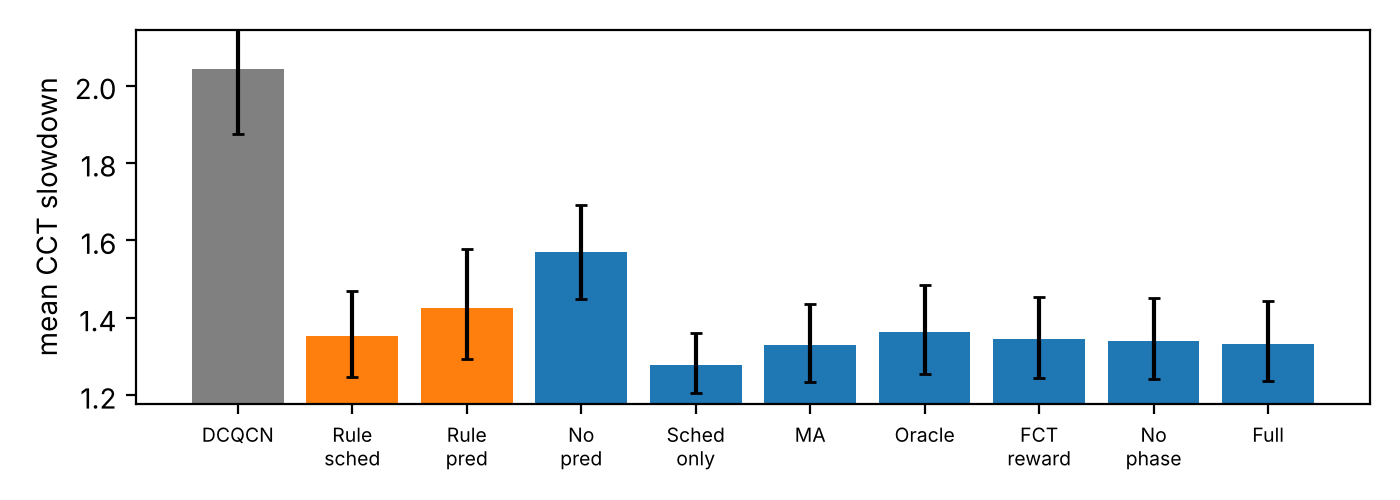
\includegraphics[width=0.85\textwidth]{figs/ablation.png}
\caption{Ablation results: mean CCT slowdown on the random test set.}
\label{fig:abl}
\end{figure*}

\textbf{Knowing the schedule is the biggest factor.} Without schedule information, the learned controller (a correction on top of DCQCN) reaches @@A_NOPRED@@, a real gain over DCQCN (@@A_DC@@) from learning alone. With the job's own schedule it reaches @@A_SCHED@@, and the hand written rule alone reaches @@A_RULE@@.

\textbf{Learning mainly removes PFC pauses.} The rule alone spends @@A_RULE_PFC@@\% of the time in PFC pause. The learned policies bring this to about zero at the same or a slightly better CCT, which is the clearest contribution of the learning step.

\textbf{Forecasting other jobs did not help.} The predictive version (@@A_FULL@@) is not better than the moving average version (@@A_MA@@) or the oracle forecast (@@A_ORACLE@@), and it is slightly worse than the schedule-aware version (@@A_SCHED@@). A perfect forecast of compute time did not help, so the limit is probably the fixed burst window heuristic and not the forecast error.

\textbf{Reward choice and phase feature.} A flow completion time reward (@@A_FCT@@) and removing the phase feature (@@A_NOPH@@) change the result only slightly, so we cannot claim that the CCT reward is clearly better in this setup.

\textbf{Quantization.} Table~\ref{tab:quant} shows that rounding the weights to 8, 6 and 4 bits does not change the result. The policy has @@QP@@ parameters and needs about @@QM@@ multiply accumulate operations per decision. Barre reports that four RISC-V cores handle ten million congestion events per second. We did not measure our policy on a NIC, so we only say that its size is in a plausible range.

\begin{table}[t]
\centering
\caption{Effect of weight quantization (predictive policy)}
\label{tab:quant}
\small
\begin{tabular}{lcc}
\toprule
\textbf{Precision} & \textbf{CCT slowdown} & \textbf{PFC (\%)} \\
\midrule
@@QUANTTAB@@
\bottomrule
\end{tabular}
\end{table}

\section{Results Analysis and Discussion}
\textbf{What the results show.} In a simulated shared link, controllers that use knowledge of the collective schedule finish iterations much sooner than reactive controllers. The predictive controller lowers the mean CCT slowdown by @@G_DC@@\% against DCQCN, @@G_HP@@\% against HPCC style, @@G_BA@@\% against Barre style and @@G_AC@@\% against ACC style on the random set, and wins on almost every scenario in both test sets. The schedule-aware version gives @@GS_DC@@\% against DCQCN and @@GS_BA@@\% against Barre style. Iteration time falls by @@ITT_G@@\% and @@ITT_GS@@\% against DCQCN, which is smaller because compute time is not affected.

\textbf{Do the results close the research gaps?} Gap 2, the missing evaluation with collective traffic and a completion time metric, is addressed inside our simulator. Gap 1, the reactive and hand-tuned behaviour, is partly addressed. Anchoring each sender to its expected fair share removes the reaction delay, and the learned correction removes PFC pauses. However, the part of Gap 1 that depends on forecasting the next burst was not confirmed. Gap 3, the choice of the optimization target, is only weakly supported, since the FCT reward was almost as good. Gap 4, the cost of learned control, is supported for size and quantization but not measured on hardware.

\textbf{Strengths.} The comparison is fair inside one simulator, uses both seen and unseen scenario families, reports confidence intervals and paired tests, and includes negative results. The policy is very small and survives 4 bit weights.

\textbf{Limitations.}
\begin{itemize}
\item The simulator is our own. It has one bottleneck, no multi-hop paths, no load balancing and no packet loss, and PFC pauses have no throughput cost. It was only sanity checked, and not validated against ns-3 or hardware.
\item The compute time traces are synthetic. The benefit of a forecaster depends on structure that we put into the data ourselves.
\item The baselines are simplified re-implementations with parameters we chose, and the results depend on them.
\item The schedule-aware anchor assumes that the sender knows its job's flow count, which needs support from the collective library. A purely NIC-local controller would not have it.
\item The learned correction gives no significant CCT gain over the hand written rule. The variants were compared on the random test set, so the ranking of variants may be slightly optimistic. The shifted set and the named scenarios were not used for choosing.
\item Our controller keeps a standing queue during bursts (Fig.~\ref{fig:trace}). The reward does not penalize queueing delay, so latency sensitive traffic sharing the link may lose some of the benefit.
\item Training used only 30 generations. Longer training may change the picture.
\end{itemize}

\textbf{Future work.} The next steps are to validate against ns-3 and ASTRA-sim, add multi-hop topologies with load balancing, use real collective traces, replace the fixed burst window with a learned concurrency estimate, and test the policy on a programmable NIC.

\section{Reproducibility}
All results come from one CPU core. The code is split into the simulator (\texttt{cnsim.py}), the scenario and forecaster module (\texttt{scen.py}), the trainer (\texttt{train.py}) and the experiment runner (\texttt{experiments.py}). Seeds are fixed: validation 999, random test 777, shifted test 888, named scenarios 100 to 109, forecaster 0. Training takes about one minute per policy, and all experiments take a few minutes. Python 3.12, NumPy, Numba, scikit-learn, SciPy and Matplotlib were used.

\section{Conclusion}
We implemented and tested a schedule-aware learned rate controller for RDMA collectives. In simulation it clearly beats DCQCN, HPCC style, Barre style and ACC style controllers on completion time and nearly removes PFC pauses. The main reason is that it knows the collective schedule, not the learning step or the compute time forecast. Our next step should be to confirm the result with a validated simulator and more realistic traffic.

\begin{thebibliography}{00}
\bibitem{barre} Y. Peng \emph{et al.}, ``Barre: Empowering simplified and versatile programmable congestion control in high-speed AI clusters,'' in \emph{Proc. USENIX ATC}, 2025, pp. 343-363.
\bibitem{spillway} M. Scazzariello \emph{et al.}, ``Avoiding cross-datacenter collective congestion via disaggregated buffering,'' arXiv:2605.11852, 2026.
\bibitem{mcc} ``Congestion control for AI workloads with message-level signaling,'' in \emph{Proc. APNET}, ACM, 2025.
\bibitem{dscc} ``DSCC: Dynamic synergistic congestion control for lossless RDMA datacenter networks,'' \emph{Computer Networks}, vol. 280, art. 112151, 2026.
\bibitem{cdcpim} ``cdcPIM: a proactive congestion control scheme for cross-datacenter RDMA networks,'' \emph{J. King Saud Univ. Comput. Inf. Sci.}, vol. 38, art. 683, 2026.
\bibitem{encc} ``ENCC: Explicit notification congestion control in RDMA,'' \emph{IEEE Trans. Netw. Serv. Manag.}, vol. 23, pp. 2415-2427, 2026.
\bibitem{dcqcn} Y. Zhu \emph{et al.}, ``Congestion control for large-scale RDMA deployments,'' in \emph{Proc. ACM SIGCOMM}, 2015.
\bibitem{hpcc} Y. Li \emph{et al.}, ``HPCC: High precision congestion control,'' in \emph{Proc. ACM SIGCOMM}, 2019.
\bibitem{acc} S. Yan \emph{et al.}, ``ACC: Automatic ECN tuning for high-speed datacenter networks,'' in \emph{Proc. ACM SIGCOMM}, 2021.
\bibitem{es} T. Salimans \emph{et al.}, ``Evolution strategies as a scalable alternative to reinforcement learning,'' arXiv:1703.03864, 2017.
\end{thebibliography}

\end{document}
